% -*- latex -*-
%%%%%%%%%%%%%%%%%%%%%%%%%%%%%%%%%%%%%%%%%%%%%%%%%%%%%%%%%%%%%%%%
%%%%%%%%%%%%%%%%%%%%%%%%%%%%%%%%%%%%%%%%%%%%%%%%%%%%%%%%%%%%%%%%
%%%%
%%%% This text file is part of the theory writeup on the
%%%% Integrative Model for Parallelism,
%%%% copyright Victor Eijkhout (eijkhout@tacc.utexas.edu) 2014-6
%%%%
%%%% cg.tex : master file for report IMP-17
%%%%
%%%%%%%%%%%%%%%%%%%%%%%%%%%%%%%%%%%%%%%%%%%%%%%%%%%%%%%%%%%%%%%%
%%%%%%%%%%%%%%%%%%%%%%%%%%%%%%%%%%%%%%%%%%%%%%%%%%%%%%%%%%%%%%%%
\documentclass[11pt,fleqn,preprint]{impreport}

\taccreportnumber{IMP-17}

\usepackage{geometry,fancyhdr,wrapfig,verbatim}

\input setup

\title[IMP CG]{The Conjugate Gradient Method in the Integrative Model for Parallelism}
\author[Eijkhout]{Victor Eijkhout\thanks{{\tt
      eijkhout@tacc.utexas.edu}, Texas Advanced Computing Center, The
    University of Texas at Austin}}

\begin{document}
\maketitle

\begin{abstract}
  We discuss the implementation of the Conjugate Gradient method
  in the Integrative Model for Parallelism (IMP).
\end{abstract}

\acresetall

\section{Power method}

As a preliminary to the \ac{CG} method, we do the power method:
\[
\begin{cases}
  x^{(0)}\equiv 1\\
  y^{(i+1)} = Ax^{(i)}\\
  x^{(i+1)} = y^{(i+1)}/\|y^{(i+1)}\|
\end{cases}
\]

\verbatimsnippet{powerqueue}

Runtime is proportional to the number of processors. This may not hold for much larger scale, since
we implement the norm as a sequence of messages, not as a collective. See~\emph{IMP-15}.

Analyze time is approximately equal
to runtime.

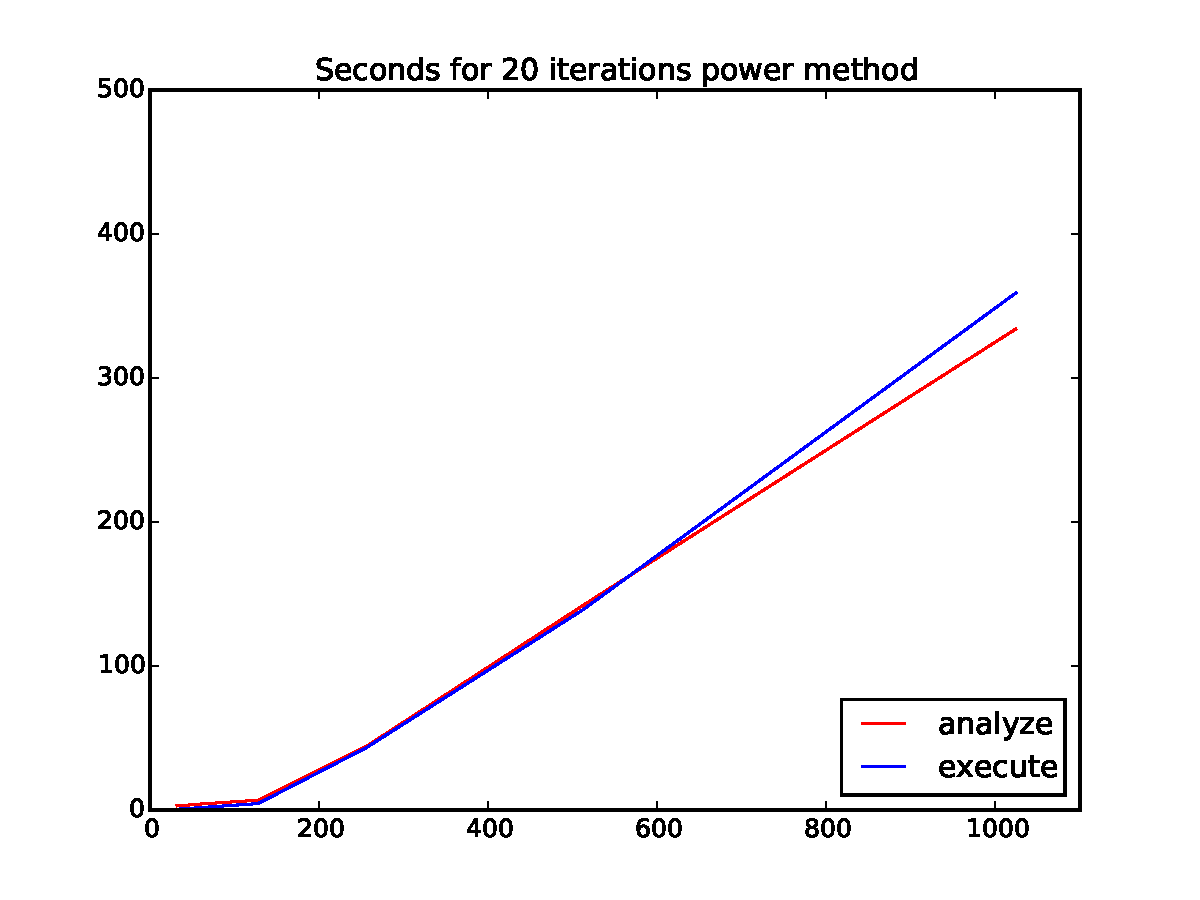
\includegraphics[scale=.5]{power_mpi_scaling}

\section{Conjugate Gradients}

The loop body of a CG iteration is easily enough written in IMP:
%
\verbatimsnippet{cgtemplate}

\subsection{Operation kernels}

This uses various kernels that are all strictly written in IMP; the slight exception
being the sparse matrix vector product which uses non-trivial skills; see \emph{IMP-13}.
Our ideal is exemplified by the copy kernel:
%
\verbatimsnippet{mpicopy}
%
which declares itself to be a copy kernel and an MPI kernel, where the general
copy kernel has all the algorithm knowledge of the copy operation:
%
\verbatimsnippet{impcopy}

Other kernels are still awaiting sophisticated application of the \indexterm{factory pattern}
to be so generalized.

\subsection{Looping}

The looping nature of CG poses a problem: we do not want to allocate as many
instances of an object (say, the search direction) as there are iterations.
Instead we create that many objects, but let them share their address spaces.
The guaranteed correctness of this relies on the execution theory of \emph{IMP-04},
but is for now based purely on programmer insight.

\subsection{Collectives}

The collectives in CG, their implementation and efficiency, are discussed in \emph{IMP-15}.

\subsection{Timing results}

A first timing run shows essentially the same scaling as a PETSc\cite{GrSm:petsc} implementation,
with slightly higher runtime. This does not surprise me or even concern me, since
everything about the IMP implementation is derived, without shortcuts or optimizations.

\heading{2016 November}
%
Stampede run, 16~cores per node, up to 200 nodes, 300k points per process
\begin{tabular}{|r|llllllll|}
  \hline
  Size&
  32&64&96&128&160&320&800&1600\\
  \hline
  PETSc&
  0.159&
  0.154&
  0.114&
  0.155&
  0.123&
  0.174&
  0.211&
  0.272\\
  IMP&
  0.250&
  0.254&
  0.256&
  0.250&
  0.262&
  0.275&
  0.411&
  0.438\\
  \hline
\end{tabular}

\includegraphics[scale=.5]{cg201611}

\section{Pipelined CG}

First (incomplete) outlined in a presentation by Gropp~\cite{Gropp:libraries},
pipelined CG is based on
introducing explicit recurrences for $M\inv r_i$ and $Ap_i$:
\[ \hbox{let $q_1=Ap_1, z_1=M\inv r_1$ be given} \]
\[
\begin{cases}
  \pi = p_1^tAp_1\\ \alpha = \rho_1 /\pi \\
  r_2 = r_1 + Ap_1\alpha\\
  z_2 = M\inv r_2\\
  \rho_2 = r_2^tz_2\\ \beta=\rho_2/\rho_1 \\
  p_2 = z_2 + p_1\beta\\
\end{cases}
\Rightarrow
\begin{cases}
  \pi = p_1^tq_1\\ \alpha = \rho_1 /\pi \\
  \begin{cases}
  r_2 = r_1 + q_1\alpha\\ z_2 = z_1+ M\inv q_1 \\
  \end{cases}\\  
  \rho_2 = r_2^tz_2\\ \beta=\rho_2/\rho_1 \\
  \begin{cases}
    p_2 = z_2 + p_1\beta\\
    q_2 = Az_2+q_1\beta\\
  \end{cases}\\  
\end{cases}
\]
We now observe that the added relations contain terms $M\inv q_1$ and
$Az_2$ that can be overlapped with inner product calculations:
\[
\begin{array}{l}
  \begin{cases}
    \hbox{overlapped:}\\
    \hbox{compute $M\inv q_1$} \\ \pi = p_1^tq_1\\ 
  \end{cases}\\  
  \alpha = \rho_1 /\pi \\
  \begin{cases}
    \hbox{in arbitrary order:}\\    
    r_2 = r_1 + Ap_1\alpha\\
    z_2 = z_1 + M\inv q_1\alpha\\  
  \end{cases}\\
  \begin{cases}
    \hbox{overlapped:}\\
    \hbox{compute $Az_2$} \\ \rho_2 = r_2^tz_2\\
  \end{cases}\\  
  \beta=\rho_2/\rho_1 \\
  \begin{cases}
    \hbox{in arbitrary order:}\\    
    p_2 = z_2 + p_1\beta\\
    q_2 = Az_2 + q_1\beta\\
  \end{cases}\\  
\end{array}
\]

\begin{figure}[ht]
  \includegraphics[scale=.5]{pipelineprods}
  \caption{Matrix-vector and vector-vector inner product in the kernel
    structure of pipelined CG}
  \label{fig:pipelineprods}
\end{figure}

Figure~\ref{fig:pipelineprods} illustrates the independence of the
$Az_2$ and $r_2^tz_2$ products: they have common inputs, common
outputs, but no causal relationship. In the IMP model, all
communications are initiated as part of the kernel that
produces~$z_2$, then overlapped with local computations.

\bibliographystyle{plain}
\bibliography{vle}

\end{document}
